\begin{frame}{Reactive walking pattern generation \only<4>{with obstacles}}
  \vspace*{-1cm}
  \begin{center}
  \scalebox{0.8}{
	\newcommand{\tetazero}{20.55}
	\newcommand{\Fkxzero}{-20}
	\newcommand{\Fkyzero}{20}
	
	\newcommand{\tetaone}{-20}
	\newcommand{\Fkxone}{5}
	\newcommand{\Fkyone}{0}
	
	\newcommand{\tetatwo}{20}
	\newcommand{\Fkxtwo}{25}
	\newcommand{\Fkytwo}{20}
	
	
	\definecolor{color1}{RGB}{1, 121, 111}% corail
	\definecolor{color2}{RGB}{27, 79, 8}% orange 
	\definecolor{color3}{RGB}{237 , 127 ,16}%
	\definecolor{color4}{rgb}{0.9,0.,0.}
	
	\begin{tikzpicture}
		\begin{axis}[xlabel=x,ylabel=y,xmin=-0.2,xmax=0.6,ymin=-0.25,ymax=0.35]
			\only<1>{
			 \addplot[black,thick=2pt,fill=gray!20]
          table{../figures/images/tikz/footstartright.dat};
			}
			\only<1-2>{
        \addplot[black,thick=2pt,fill=gray!20]
          table{../figures/images/tikz/footstartleft.dat};       
			}
			\only<2-3>{
        \addplot[black,thick=2pt,fill=gray!20]
          table{../figures/images/tikz/foot2.dat};
      }
      \only<3-4>{
        \addplot[black,thick=2pt,fill=gray!20]
          table{../figures/images/tikz/foot3.dat};
      }
      \only<4-5>{
        \addplot[black,thick=2pt,fill=gray!20]
          table{../figures/images/tikz/foot4.dat};
			}
			\only<5-6>{
        \addplot[black,thick=2pt,fill=gray!20]
          table{../figures/images/tikz/footendleft.dat};
			}
			\only<6>{
        %\addplot[black,thick=2pt,dashed,fill=white,opacity=0.5]
        \addplot[black,thick=2pt,fill=gray!20]
          table{../figures/images/tikz/footendright.dat};
			}
	    \only<9->{
			  \addplot[black,thick=5pt,fill=gray!20]
			    	table{../figures/images/tikz/footconstraint.dat}; 
  			  \addplot[dashed,black,thick=5pt,fill=gray!20]
			    table{../figures/images/tikz/foot.dat};
			  \addplot[black,very thick,fill=gray!20]
			    table{../figures/images/tikz/footmargin.dat};
	    }
	    	\only<7-8>{
	    	  \addplot[dashed,black,thick=2pt,fill=gray!10,opacity=0.5]
          table{../figures/images/tikz/footstartright.dat};
        \addplot[dashed,black,thick=2pt,fill=gray!10,opacity=0.5]
          table{../figures/images/tikz/footstartleft.dat};
        \addplot[dashed,black,thick=2pt,fill=gray!10,opacity=0.5]
          table{../figures/images/tikz/foot2.dat};
        \addplot[dashed,black,thick=2pt,fill=gray!10,opacity=0.5]
          table{../figures/images/tikz/foot3.dat};
        \addplot[dashed,black,thick=2pt,fill=gray!10,opacity=0.5]
          table{../figures/images/tikz/foot4.dat};
        \addplot[dashed,black,thick=2pt,fill=gray!10,opacity=0.5]
          table{../figures/images/tikz/footendleft.dat};
        \addplot[dashed,black,thick=2pt,fill=gray!10,opacity=0.5]
          table{../figures/images/tikz/footendright.dat};
	    	}
	    	\only<8->{
			  % com
			  \addplot[color1,thick=2pt] table[x index= 0,y index=1]
			    	{../figures/images/tikz/table.dat};
			}
	    	\only<7->{
	      % cop
			  \addplot[color2,thick=5pt] table[x index= 2,y index=3]
			    	{../figures/images/tikz/table.dat}; 
			}
		\end{axis}
	\end{tikzpicture}
	}
	\end{center}
\end{frame}


\begin{frame}{Reactive walking pattern generation \only<4>{with obstacles}}
  \only<4>{\blfootnote{\textbf{Naveau} et al., RA-L 2016}}
  \begin{minipage}{0.48\textwidth}
    Optimization problem solved :
    \vspace*{-0.3cm}
    \begin{equation*}
      \begin{aligned}
        \min_{{\bf U}_k} 
        \sum_{i=0}^{j=4} w_i L_i({\bf U}_{k}) & \\
        {\bf X}_{k+1} = {\bf A}{\bf X}_{k} + {\bf B} {\bf U}_k & \\
        \underline{\bf P} < {\bf P}\only<4>{{\color{red}{({\bf U}_k)}}} {\bf U}_k  < \overline{\bf P}& \\
      \end{aligned}
    \end{equation*}
    with ${\bf U}_k=\begin{pmatrix} \dddot{\bf C}^x_k \; {\bf F}^x_k\; \dddot{\bf C}^y_k \;{\bf F}^y_k \;\only<4>{\color{red}{{\bf \Theta}_k^\mathit{f}}}\end{pmatrix}^T$ \\
  \end{minipage}
  %
  \begin{minipage}{0.48\textwidth}
    \only<1-3>{
      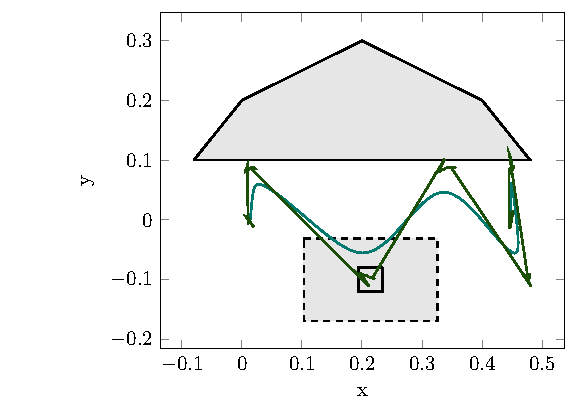
\includegraphics[width=\textwidth]{./images/tikz/convexHulls2}
    }
    \only<4>{
      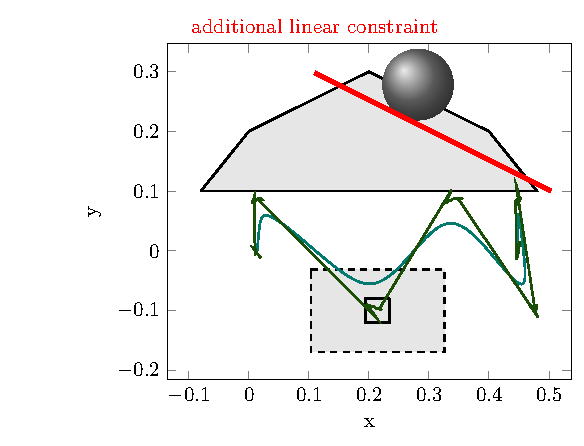
\includegraphics[width=\textwidth]{./images/tikz/convexHullsplusObstacles2}
    }
  \end{minipage}\\
  \vspace*{-0.5cm}
  \begin{center}
  \only<1>{
    {
      \small $L_1({\bf U}_k)$ : linear velocity tracking
%      \begin{equation*}
%        \text{linear velocity tracking : }
%        L_1({\bf U}_k) = \lVert \dot {\bf X}_{k} - {\bf X}_{k}^{ref} \rVert^2_2
%        +  \lVert \dot {\bf Y}_{k} - {\bf Y}_{k}^{ref} \rVert^2_2 
%      \end{equation*}
    }
  }
  \only<2>{
    {
      \small $L_2({\bf U}_k)$ : control norm
%      \begin{equation*}
%        \text{control norm : }
%        L_2({\bf U}_k) = \lVert \dddot {\bf X}_{k} \rVert^2_2
%        + \lVert \dddot {\bf Y}_{k} \rVert^2_2
%      \end{equation*}
    }
  }
  \only<3>{
    {
      \small $L_3({\bf U}_k)$ : balance criteria
%      \begin{equation*}
%        \text{balance criteria : }
%        L_3({\bf U}_k) = \lVert {\bf X}_{k}^{f} - CoP_{k+1}^{x} \rVert^2_2 +
%        \lVert {\bf Y}_{k+1}^{f} - CoP_{k+1}^{y} \rVert^2_2 
%      \end{equation*}
    }
  }
  \only<4>{
    {
      \small $L_4({\bf U}_k)$ : angular velocity tracking
%      \begin{equation*}
%        \text{angular velocity tracking : }
%        L_4({\bf U}_k) = \lVert {\bf \Theta}_{k} 
%        - \int {\bf \Theta}_{k}^{ref} dt \; \rVert_2^2 
%    \end{equation*}
    }
  }
  \end{center}
  
\end{frame}

%%%%%%%%%%%%%%%%%%%%%%%%%%%%%%%%%%%%%%%%%%%%%%%%%%%%%%%%%%%%%%%%%%%%%%%%%%%%%%%


\begin{frame}{SQP Solver}

\begin{itemize}
\item Original nonlinear problem :
  \begin{align*}
    \min_{\color{txtcolor2}{\bf U}_k}  \quad & L({\color{txtcolor2}{\bf U}_k}) \\
    \text{s.t.} \quad & \underline{\bf P} \leq \tilde{\bf P}({\color{txtcolor2}{\bf U}_k}) \leq \overline{\bf P}
  \end{align*}
\item QP approximation :
  \begin{align*}
    \min_{{\color{txtcolor5}{\bf \Delta U}_k}} \quad &
    g({\bf U}_{k-1}) {\color{txtcolor5}{\bf \Delta U}_k} +
    \frac{1}{2} {\color{txtcolor5}{\bf \Delta U}_k}^T H({\bf U}_{k-1}) {\color{txtcolor5}{\bf \Delta U}_k} \\
    \text{s.t.} \quad & \underline{h} - h_{k-1} \leq J({\bf U}_{k-1}) {\color{txtcolor5}{\bf \Delta U}_k} \leq \overline{h} - h_{k-1}\\
    {\color{txtcolor2}{\bf U}_k} =& {\bf U}_{k-1} + \alpha {\color{txtcolor5}{\bf \Delta U}_k}
  \end{align*}
\end{itemize}
\end{frame}

%%%%%%%%%%%%%%%%%%%%%%%%%%%%%%%%%%%%%%%%%%%%%%%%%%%%%%%%%%%%%%%%%%%%%%%%%%%%%%%

\begin{frame}{Dynamic Filter}
\blfootnote{\textbf{Naveau}, Kudruss et al., Humanoids 2014}
\vspace*{-1cm}
  \begin{center}
    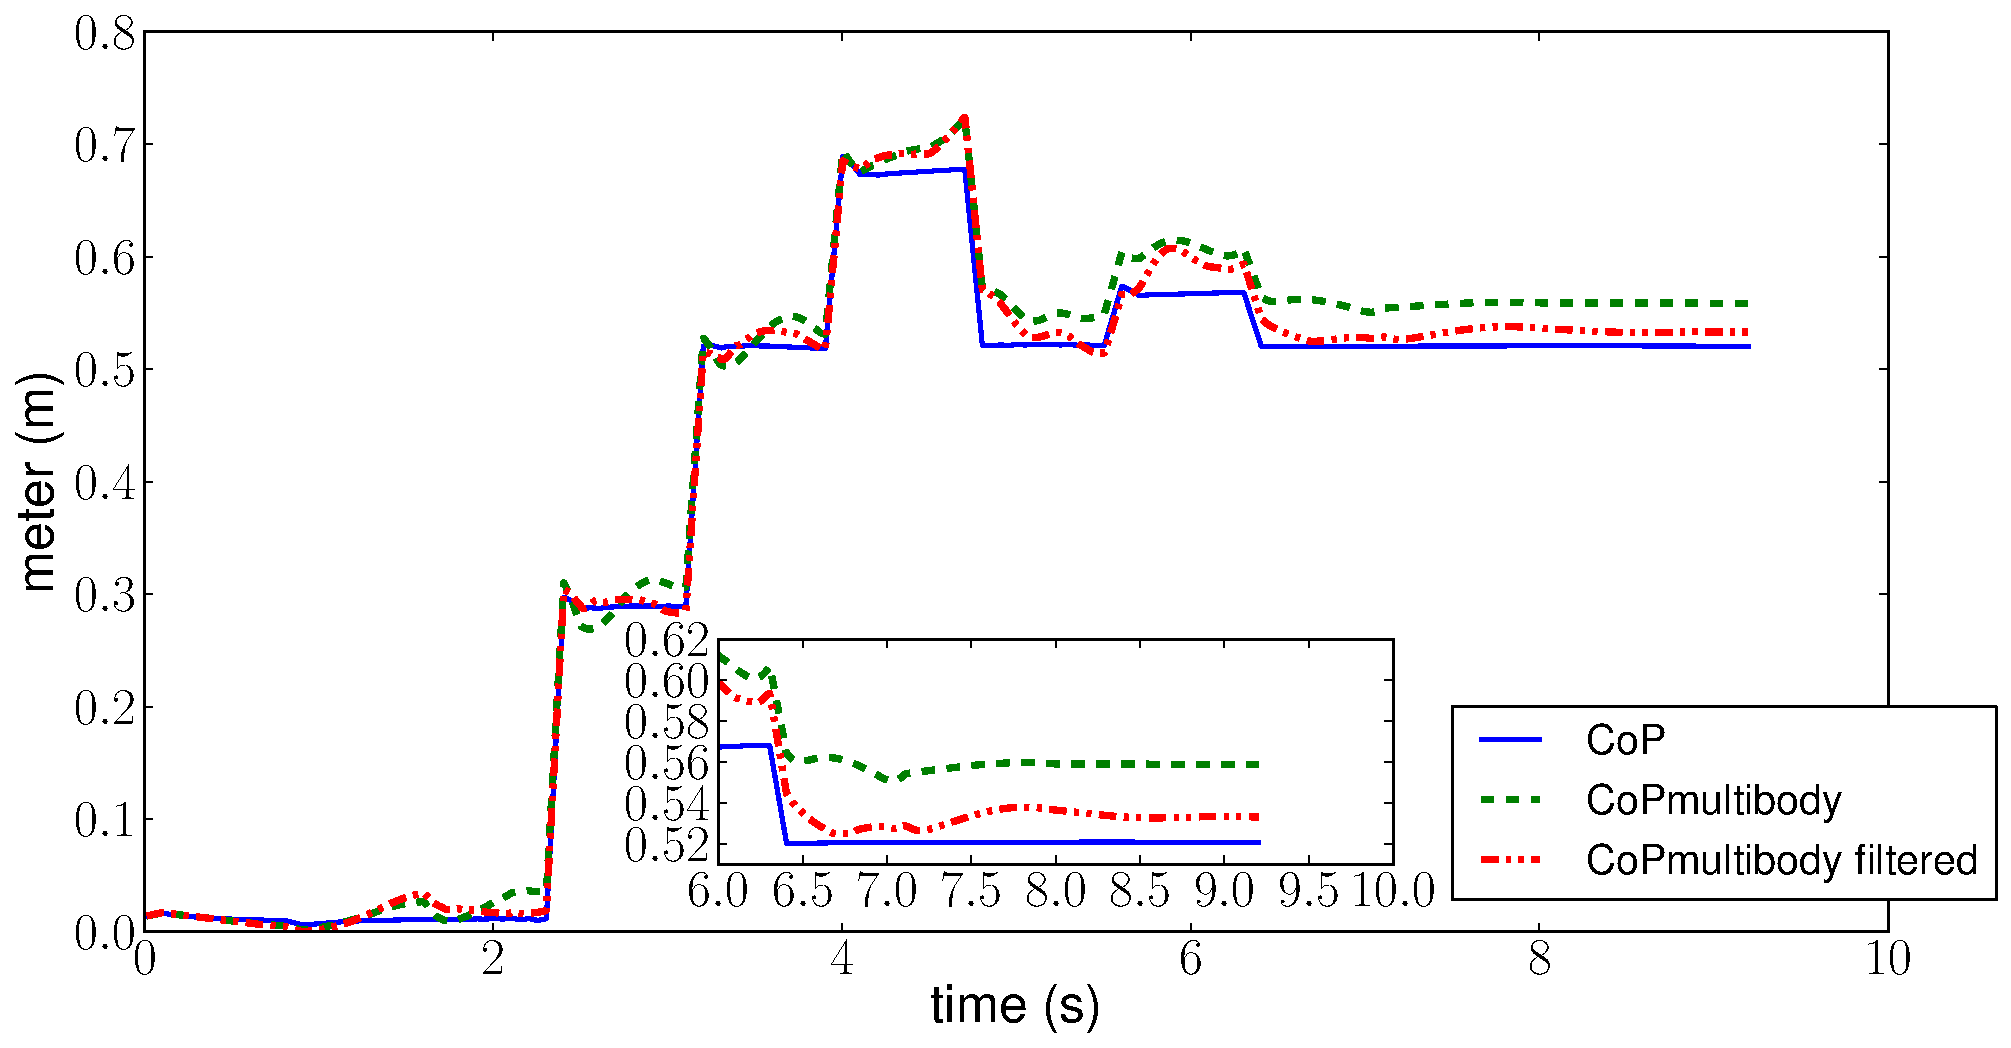
\includegraphics[height=0.8\textheight, keepaspectratio]
      {./figures/nmpc_walkgen/copmbpres.pdf}    
  \end{center}
\end{frame}

%%%%%%%%%%%%%%%%%%%%%%%%%%%%%%%%%%%%%%%%%%%%%%%%%%%%%%%%%%%%%%%%%%%%%%%%%%%%%%%

\begin{frame}{Feedback Scheme}

\begin{center}
  \hspace*{-1cm}
  \scalebox{0.7}{%!TEX root = ../../14-icra-RealTimeNMPC.tex

\tikzstyle{block} = [draw, fill=blue!20, rectangle,
    minimum height=2em, minimum width=5em, align=center]
\tikzstyle{sum} = [draw, fill=blue!20, circle, node distance=1cm]
\tikzstyle{input} = [coordinate]
\tikzstyle{output} = [coordinate]
\tikzstyle{pinstyle} = [pin edge={to-,thin,black}]

% The block diagram code is probably more verbose than necessary
\begin{tikzpicture}[auto, node distance=2cm,>=latex]

    % We start by placing the blocks
    \node [input]  at (0.0, 0.0) (input)  {};
    \node [input]  at (3, 0.0) (velocity) {};
    \node [input]  at (7.2, -2.8) (feedback)  {};
    \node [input]  at (16, -2.8) (feedback2)  {};
    \node []    at ( 0.0, 0.0) (sumin)  {};
    %\node [output]    at ( 15, 0.0) (sumout) {};
    \draw [fill=green,opacity=.2,text opacity=1] (0.1,1.5) rectangle (12.6,-2.0);
    \node at(10,-1.7) {\textcolor{green!20!black!100}{Stack of Tasks}};

%    \node [block] at (4.6,-1.7) (lwc) {
%        Left Wrist\\
%        Hybrid\\
%        Controller        
%    };

%    \node [block] at (1.7,0.0) (walking) {
%        Walking \\
%        Task    
%    };

    \node [block] at (1.7,0) (wpg) {
        Walking\\
        Pattern\\
        Generator
    };
    \node [block, fill=green!30!black!80] at (5.2,0) (dyn) {
        Dynamic\\
        Filter
    };
    \node [block] at (8.5,0) (ttt) {
        Task for\\
        Trajectory\\
        Tracking
    };    
    \node [block] at (11.5,0) (qp) {
        HQP\\
        solver
    };
    \node [block] at (15, 0) (system) {
    		Robot Hardware\\
    		{\footnotesize Simulation/Robot}\\
    		and\\
    		{\footnotesize motion capture system}
    	};

    % PATHS
    	% Forward chaine
%    \draw [draw,-] (input) -- node {\small ${\mathbf{p}}^{\,{\text {ref}}}$} (walking);
    
    \draw [draw,->] ([xshift=-2cm]wpg.west) -- node {\small ${\mathbf v}^{\,{\text{ref}}}$} (wpg);
%    \draw [draw,- ] (walking) -- node {} (velocity);
%    \draw [draw,->] (velocity) |- node {} (lwc);
%    \draw [->] (wpg) -- node {\small $c^{ref},f^{ref}$} (dyn);
%    \draw [->] (dyn) -- node {\small $\tilde{c}^{\,ref},f^{ref}$} (sot);
    \draw [->] (wpg) -- node [text width=1cm]{\small ${\mathbf{p}_{com}}^{\,{\text {ref}}}$ ${\mathbf{p}_{foot}}^{\,{\text {ref}}}$} (dyn);
    
    \draw [->] (dyn) -- node [text width=1cm]{\small ${\tilde{\mathbf{p}}_{com}}^{\,{\text {ref}}}$ ${\mathbf{p}_{foot}}^{\,{\text {ref}}}$} (ttt);
    
    \draw [->] (ttt) -- node [text width=1cm]{
    \small Tasks
    } (qp);
    \draw [->] (qp) -- node [text width=0.6cm]{\small ${\mathbf q}^{\,{\text{ref}}}$ $\dot{{\mathbf q}}^{\,{\text{ref}}}$} (system);
    
%    \draw [->] (lwc) -| node [near start, above]{\small ${\mathbf{p}_{lw}}^{\,{\text {ref}}}$} (ttt);
    %\draw [->] (system) -- node {} (sumout);

    % Feedback chaine
    \draw [- ] ([xshift=+0.8cm]dyn.east) |- node {}
               ([xshift=-0.5cm,yshift=-1.0cm]wpg.west);
    \draw [->] ([xshift=-0.5cm,yshift=-1.0cm]wpg.west) |- node {}
               ([yshift=-0.2cm]wpg.west);
    
%    \draw [- ] (system.east)    -| node {} (feedback2);
%    \draw [- ] (feedback2)  -- node [above]{\small $\mathbf{f}_{lw},\mathbf{p}_{w},\mathbf{p}_{lw},\mathbf{p}_{f}$} (feedback);
%    \draw [->] (3.0,-2.8) |- node [near start, above]{} ([yshift=-0.2cm]lwc.west);
%    \draw [->] (feedback) |- node [below=0.7cm, right]{\small $\mathbf{p}_{ch}$} ([yshift=-0.2cm]walking);

%    \draw [->] (dyn) -| node[above right] {\small $\hat{c}^{\,x,y,\theta}$, $\hat{f}^{\,\,x,y,\theta}$} (wpg);
\end{tikzpicture}
}
\end{center}

\end{frame}

%%%%%%%%%%%%%%%%%%%%%%%%%%%%%%%%%%%%%%%%%%%%%%%%%%%%%%%%%%%%%%%%%%%%%%%%%%%%%%%

\begin{frame}{Experiment on HRP2}
  \begin{center}
    \movie[autostart,loop]{
    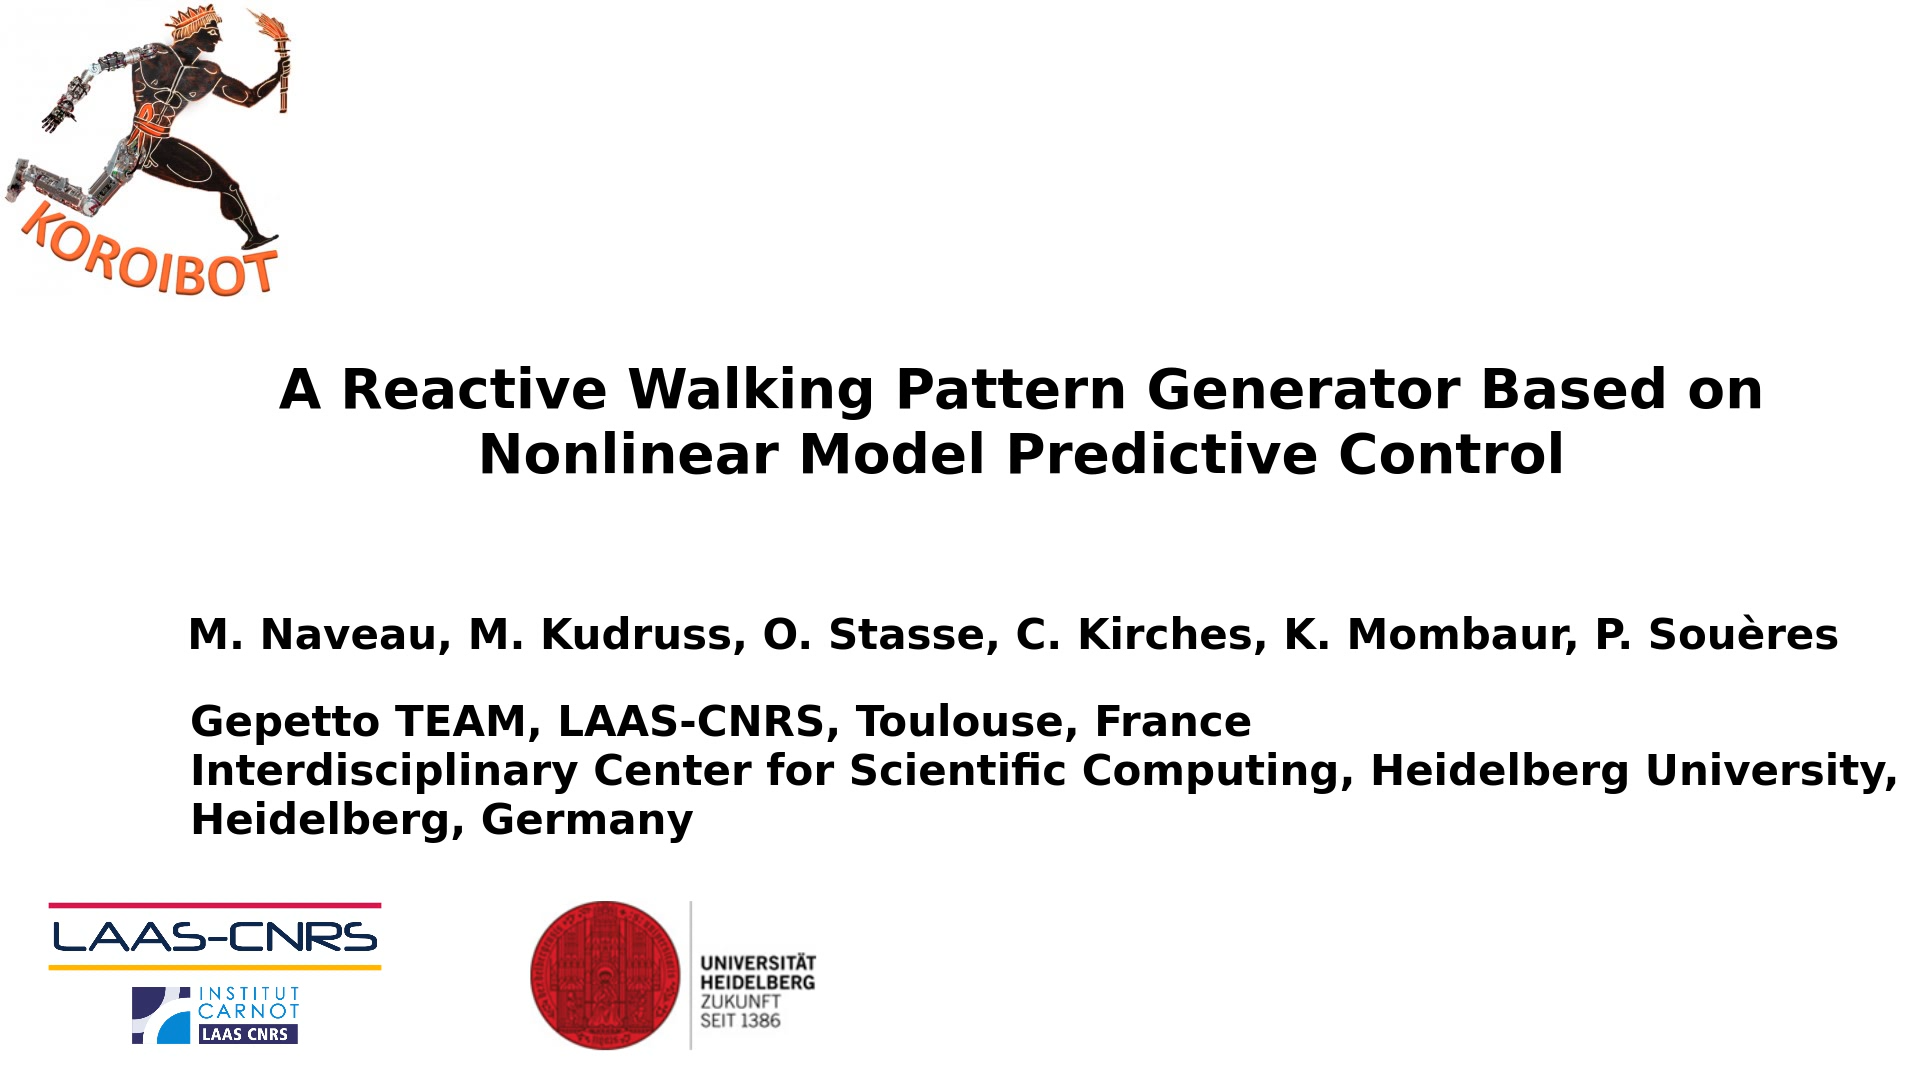
\includegraphics[width=0.85\linewidth, keepaspectratio]
      {16-raletter-NMPC-v19.png}    
    }  
    {videos/16-raletter-NMPC-short.mp4}
  \end{center}
\end{frame}

%%%%%%%%%%%%%%%%%%%%%%%%%%%%%%%%%%%%%%%%%%%%%%%%%%%%%%%%%%%%%%%%%%%%%%%%%%%%%%%

